%!TEX root = main.tex
\section{Design of DawnPiper}
\label{sec:design}
\subsection{Design Overview}
The overall architecture of DawnPiper is shown in Figure~\ref{fig:sys_arch},
which includes three modules for the partition of the pipeline parallelism.
We will give them a brief introduction next.

\begin{figure*}[t]
  \centering
  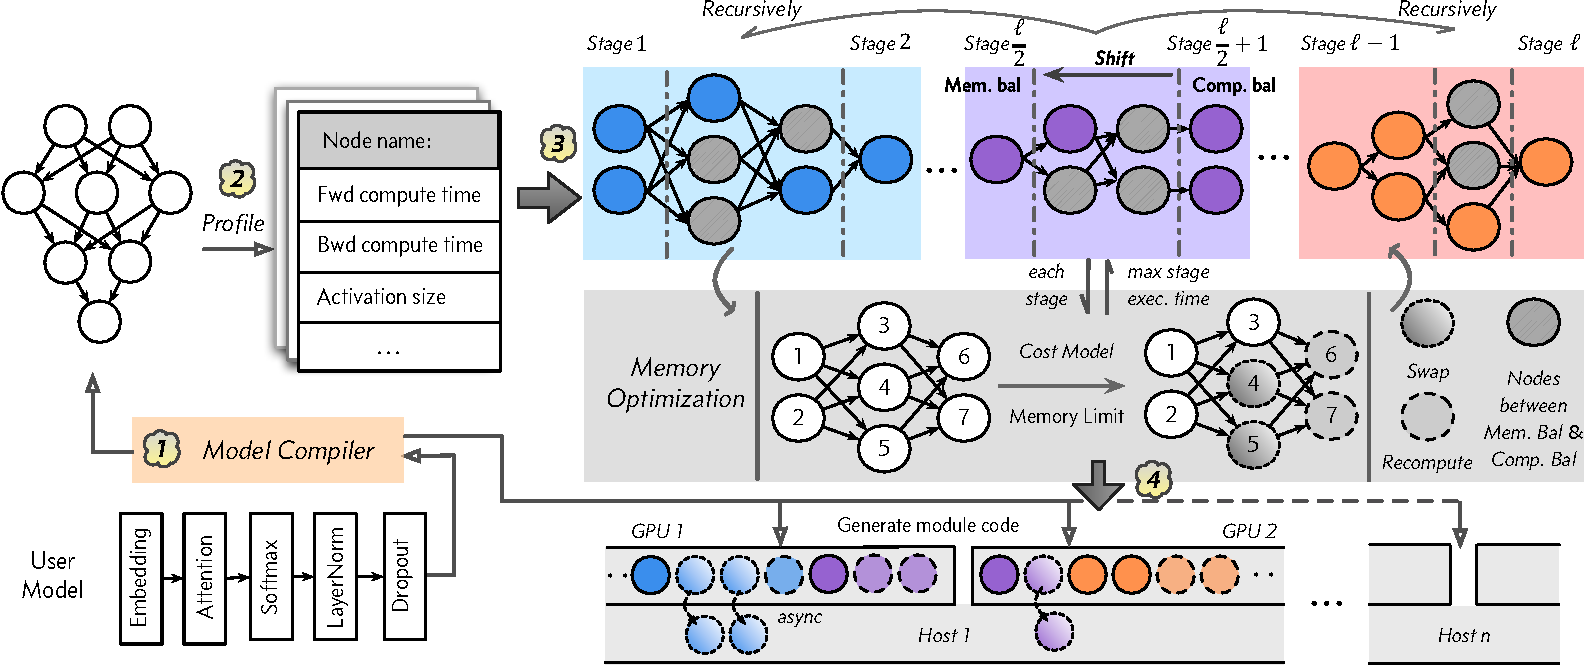
\includegraphics[width=0.95\linewidth]{pp-opt-arch-crop.pdf}
  \caption{DawnPiper System Architecture}
  \label{fig:sys_arch}
\end{figure*}

\textbf{Compiler:} Once the user submits a model for pipeline parallelism,
the \emph{compiler} obtains its fine-grained computation graph via DL compilation.
The computation graph includes all operators (nodes) in the training process and
the connection information between nodes.
This compilation-based approach allows subsequent model partitioning
and memory optimization to be performed
on this fine-grained computation graph.
In the meantime, the model code of each stage after the model partitioning
can be automatically generated based on the partitioned sub-graphs,
eliminating the need for manual involvement in the process,
making the system highly versatile and practical.

\textbf{Profiling:} This module is responsible for acquiring the
execution metadata of each node for the fine-grained computation graph.
For a node \emph{n}, its execution metadata data include the forward computation time $t_f^n$,
backward computation time $t_b^n$, the activation memory size $m_a^n$,
the size of the model parameters and optimizer states at this node $m_p^n$,
and the list of saved tensor ${st}^n$.
Based on the nodes dependencies information,
the memory size that needs to be released at each node can be inferred as $m_d^n$.
With the above information, the computation time, peak memory usage,
and inter-stage communication volume of each stage can
be easily deduced when partitioning the model at any nodes.
Meanwhile, the memory optimization policy could also be decided using the metadata.

\textbf{Pipeline Partitioning:} This module is responsible for the pipeline partition.
The basic idea is limiting the pipeline partition range between
the positions of the compute-balance and memory-balance.
When traversing each possible partition positions,
the memory optimization module will identifie the minimum
memory optimization cost that allows each stage's training process to
meet the GPU memory capacity limit for a given model partitioning.
After traversing all model partition positions,
the target partition strategy is the one with the
smallest time of the longest execution stage.

% \textbf{Memory Optimization Module:} This module identifies the minimum memory optimization cost method
% that allows the model execution process in each stage to meet the GPU memory capacity limit for each
% pipeline partitioning method obtained by traversing every partition position in the aforementioned
% pipeline partitioning module. This allows the deduction of the longest execution time stage under
% this partition strategy and records the corresponding execution time.

Next, we will dive into the details of the pipeline parallelism partition and memory optimization algorithms.

\subsection{Pipeline Terminology and Partition Theorem}
The number of the pipeline stages is denoted as $\ell$,
For a pipeline stage $x$, $x \in [1, \ell]$,
the set of computation nodes it contains is defined as $\mathcal{N}_x$.
The computation time of this stage can be obtained
by adding the forward and backward computation times
of all nodes in the set, as shown in Equation (3.1).
\begin{align}
  T_x=\sum_{n \in \mathcal{N}_x}\left(t_f^n+t_b^n\right)
\end{align}

The peak memory usage of a stage can be calculated according
to the set of nodes in the stage and the pipeline scheduling method.
The optimal performance partition is to make the
processing time of all stages as close as possible.
Since the inter-stage communication mentioned earlier
can be minimal and can be executed concurrently with computation,
the goal is to minimize the computation time of the longest stage,
i.e., the stage with the longest execution time, among all partitioning strategies,
while the peak GPU memory usage of all stages are less than the GPU memory capacity,
that is $minimize\ \max_{1 \leq x \leq \ell} T_x$.

Due to the fine-grained computation graph obtained by DL compilation,
the entire search space will grow exponentially and become very large
if we consider all possible partition positions coupled with each
possible memory optimization combinations.
Therefore, it is necessary to eliminate unreasonable
pipeline partitions to shrink the total search space.
We propose a partition theorem to restrict the partition space
by leveraging the memory usage features mentioned above.

\textbf{Theorem:} Given a model that needs to be divided into two pipeline stages,
the optimal pipeline partition must exist in the closed interval between the compute-balance and
memory-balance partition positions when the following three conditions are met:
1) The computation time and memory usage during the forward propagation
show a monotonically increasing trend as operations are continuously scheduled;
2) The time required for inter-stage communication is
always less than the computation time of the stage;
3) The memory optimization targets are evenly distributed throughout the entire model.

\textbf{Proof:} For convenience, let's illustrate with the simplest example of a
2-stage pipeline parallelism, and the proof can be extended to more than 2 stages accordingly.
The pipeline compute-balance and memory-balance partition positions
are denoted as $\rho_{cb}$ and $\rho_{mb}$, respectively.
For the 1F1B computation scheduling in the asynchronous pipeline,
since the earlier stages need to store more activations and parameters memory,
the position of $\rho_{cb}$ is usually further to the right than $\rho_{mb}$
(the case where the positions are reversed can also be proven using the following method).
As shown in the model partitioning in step 3 of Figure~\ref{fig:sys_arch},
if the partition position is moved further to the right from $\rho_{cb}$,
which means more computation nodes are assigned to the first stage,
due to the feature of monotonicity of computation time and memory usage,
and the negligible communication overhead,
the computation time and peak memory usage of the first stage are increasing,
while that of the second stage are decreasing.
Since the memory optimization targets are essentially
evenly distributed throughout the entire model structure,
there will not be a stage with smaller memory usage
that requires a greater memory optimization cost to meet the GPU memory limit.
This leads to the fact that no matter whether memory optimization is needed,
the first stage is definitely the longest stage,
and it exceeds the computation time of the longest stage under the compute-balance partition.
So the pipeline parallel training performance is continuously
decreasing as the partition position moves from $\rho_{cb}$ to the right.
Similarly, if the partition position is moved further to the left from $\rho_{mb}$,
then the second stage is definitely the longest computation time stage,
and it will continuously increase as the movement progress.

\subsection{Compute and Memory Balance Partition}
In this section, we will introduce how to find the compute-balance and memory-balance partition positions.
The basic process is to traverse the nodes in the compute graph according to the execution order,
continuously accumulating the forward/backward computation time or the memory consumption.
Since the memory footprint of each stage needs to consider the
stage number in asynchronous pipeline parallelism,
while the computaiton time of each stage can be simply added,
we only give the memory-balance partition algorithm for PipeDream
in this section which is shown as Algorithm~\ref{alg:mem-ba}.

Before the algorithm begins,
we first traverse the compute graph to calculate the depth of each node.
Nodes with the same depth are sorted by the start time of forward computation,
and this node set is denoted as $\mathcal{N}_\mathcal{G}$ for the algorithm input.
Besides, the inputs also include the GPU peak memory usage $M_\mathcal{G}$ and the number of pipeline stages $\ell$.
The output of the algorithm is the partition positions of each stage $\rho_x$.
The ratio of activations and parameters copies that need to be stored from the first stage
to the last stage is $\ell:(\ell-1):(\ell-2):\cdots:1$ in PipeDream.
If the peak memory usage corresponding to each stage for a micro-batch is defined as $M_x$,
in order to make the peak memory usage of all stages equal,
the following equation must exist:
\begin{align}
  \ell \times M_1=\cdots=(\ell-x+1) \times M_x=\cdots=M_{\ell}
\end{align}
% \ell \times M_1=(\ell-1) \times M_2=\cdots=(\ell-x+1) \times M_x=\cdots=M_{\ell}
Based on this equation, the $M_x$ of each stage can be calculated,
as shown in lines 2-5 and line 12 of Algorithm~\ref{alg:mem-ba}.
In this way, the algorithm can continuously traverse the nodes,
first adding the activation memory, parameter memory, and optimizer state memory size of the node,
and then determining whether it exceeds the previously recorded peak memory size.
Next, subtract the memory size that needs to be released at this node,
and continue to repeat until the peak memory size reaches the current stage's $M_x$.
At this point, current node is the position where this stage needs to be partitioned.
It should be noted that for the sake of convenience in description,
the partition position is a single node,
but it is usually a set of nodes in practice.

\begin{algorithm}
  \SetKwInOut{Input}{Input}
  \SetKwInOut{Output}{Output}
  $x \leftarrow 1,cur\_mem \leftarrow 0,peak\_mem \leftarrow 0$\;
  \For{$i$ in $[0,\ell)$}
  {
    $sum += \ell \div (\ell-i)$\;
  }
  $M_x \leftarrow M_\mathcal{G} \div sum$\;
  \For{$n$ in $N_\mathcal{G}$}
  {
    $cur\_mem += m_a^n + n_p^n$\;
    $peak\_mem \leftarrow \max(cur\_mem,peak\_mem)$\;
    $cur\_mem -= m_d^n$\;
    \If{$peak\_mem \ge M_x$}
    {
      $\rho_x \leftarrow n,x \leftarrow x + 1$\;
      $M_x \leftarrow (\ell \div (\ell -x + 1) \times M_1)$\;
      $cur\_mem, peak\_mem \leftarrow 0$\;
      \If{$x == \ell$}
      {
        \textbf{break}\;
      }
    }
  }
\caption{Memory balance partition in PipeDream}
\label{alg:mem-ba}
\end{algorithm}

\subsection{Binary Pipeline Parallel Partition}
If the peak memory footprint of all stages at compute-balance partition
are less than the GPU memory capacity,
then this is already the optimal pipeline partitioning
in terms of performance.
Otherwise, it is necessary to continuously move the partition position from
$\rho_{cb}$ the towards the $\rho_{mb}$ or take memory optimization
operations to reduce memory usage.
Both of these two methods will change the execution time of a stage,
it is difficult to analyze which partition and memory optimization strategy
will produce the optimal pipeline parallel performance.
Therefore, it is necessary to perform a combination traversal of the possibilities.
During the process, given a pipeline partition, the goal of memory optimization for each stage
is to minimize the memory optimization cost while meeting the GPU memory capacity limit.
Define the minimum memory optimization cost time corresponding to stage $x$ as $T_x^{moo}$,
then the objective of the pipeline partition with memory optimization
is to $minimize\ \max_{1 \leq x \leq \ell} (T_x + T_x^{moo})$ .

It should be noted that during the process of moving from the $\rho_{cb}$
to the $\rho_{mb}$, if the peak memory usage of the adjacent two stages after partitioning
are less than the GPU memory limit without memory optimization,
then there is no need to continue to traverse subsequent partition possibilities.
This conclusion can also be proven using the above theorem.
In simple terms, if the partition position continues to move at this time,
the computation time and memory usage of the stage
with more computation time will continue to increase.
Regardless of whether it still needs memory optimization,
its total computation time will continuously increase
and exceed the longest execution stage's computation time at the current partition position.
% Therefore, the shortest time of the longest execution stage during the partition position movement
% will definitely not appear behind this partition position.

Based on the above discussion,
the naive idea is to start from the $\rho_{cb}$
of the first stage and continuously move towards the $\rho_{mb}$ for traversal.
For each position, calculate the $\rho_{cb}$ and
$\rho_{mb}$ of the subsequent $\ell - 1$ stages
until the last two adjacent stages.
Then we use memory optimization to obtain the minimal cost for each stage.
By that, we can know the computation time of the longest execution stage for the current partition positions.
After traversing all partition positions,
we can find the optimal partition and memory optimization strategy.
% is the strategy corresponding to the minimum computation time of the longest execution stage.
Although the range of each partitioning operation is restricted between the $\rho_{cb}$
and the $\rho_{mb}$, the search space increases exponentially with the number of pipeline stages.
Therefore, to cope with the pipeline parallel partitioning of longer stages,
we adopts a binary pipeline parallel partitioning method,
which first enumerates from the middle stage of the pipeline.
Each time the middle is divided, the left and right parts are regarded as two stages
to achieve compute-balance and memory-balance.
In this way, the shortest computation time of the longest execution stage
on the left and right parts at each binary partitioning can be found level by level.
When the outermost level finishes traversing all possible partition positions,
then the optimal partition strategy can be found.
By that, the complexity of the partition algorithm is successfully
reduced to $\mathcal{O}(\varphi^{log\ell})$,
where $\varphi$ represents the number of possible partitions that
need to be traversed from the $\rho_{cb}$ to the $\rho_{mb}$.
This number is far smaller than the total number of nodes in the model.
Take the BERT for example, its total nodes are more than 1000,
in which the number of nodes in this range are less than 100.
% and the communication optimization method to be introduced below can further reduce the
% possible partition positions.
The overall process of this partitioning method is shown in Algorithm~\ref{alg:binary-partition}.

\begin{algorithm}[t]
  \SetKwInOut{Input}{Input}
  \SetKwInOut{Output}{Output}
  \SetKwFunction{Fmain}{BinaryPartition}
  \SetKwFunction{Fadj}{AdjacentPartition}
  \SetKwProg{Fn}{Function}{:}{}
  \Fn{\Fadj{$\mathcal{N},sid$}}
  {
    $\rho_{cb},\rho_{mb} \leftarrow CompMemBalPartition(\mathcal{N}, sid, \ell)$\;
    \If{$\max_{sid \le x \le sid+1} ((\ell-x+1) \times M_x^{\rho_{cb}}) < M$}
    {
      \textbf{return} $\max_{sid \le x \le sid+1} T_x^{\rho_{cb}}$\;
    }
    $sorted\_pps \leftarrow IdentifyAndSort(\rho_{cb},\rho_{mb})$\;
    \For{$\rho \leftarrow sorted\_pps$}
    {
      $mopt_l,min\_t_l \leftarrow MemOpt(\mathcal{N}_{sid},M)$\;
      $mopt_r,min\_t_r \leftarrow MemOpt(\mathcal{N}_{sid+1},M)$\;
      $mopt \leftarrow mopt_l \cup mopt_r$\;
      $par\_dict[\rho] \leftarrow (\max(min\_t_l,min\_t_r),mopt)$\;
      \If{$!mopt$}
      {
        \textbf{break}\;
      }
    }
    \textbf{return} $\min(par\_dict)$
  }
  
  \Fn{\Fmain{$\mathcal{N},\mathcal{L},\mathcal{R}$}}
  {
    \If{$\mathcal{R}-\mathcal{L}==1$}
    {
      \textbf{return} $AdjacentPartition(\mathcal{N},\mathcal{L})$\;
    }
    $mid \leftarrow (\mathcal{L}+\mathcal{R}) /div 2$\;
    $\rho_{cb},\rho_{mb} \leftarrow CompMemBalPartition(\mathcal{N}, mid, \ell)$\;
    \For{$\rho \leftarrow sorted\_pps$}
    {
      $\rho_l,mopt_l,min\_t_l \leftarrow BinaryPartition(\mathcal{N}_{\mathcal{L}},\mathcal{L},mid)$\;
      $\rho_r,mopt_r,min\_t_r \leftarrow BinaryPartition(\mathcal{N}_{\mathcal{R}},mid+1,\mathcal{R})$\;
      $mopt \leftarrow mopt_l \cup mopt_r$\;
      $par\_dict[\rho] \leftarrow (\max(min\_t_l,min\_t_r),mopt)$\;
      \If{$!mopt$}
      {
        \textbf{break}\;
      }
    }
  }

\caption{Binary pipeline parallel partition}
\label{alg:binary-partition}
\end{algorithm}

The \texttt{AdjacentPartition} function of the Algorithm~\ref{alg:binary-partition}
describe how to find the partitioning and memory optimization strategy
that minimizes the difference in computation time between two adjacent stages.
The $\rho_{cb}$ and $\rho_{mb}$ of two adjacent stages
can be easily found by modifying Algorithm~\ref{alg:mem-ba}.
The line 7-8 describes the memory optimization process for the adjacent stages which
finds the policy that can achieve the shortest execution time under the memory limit.
The line 10-13 means the traversal process can exit in advance
when there is no memory optimization for the two stages.
This function finally returns the optimal partition and memory optimization strategies
and the corresponding execution time of the longer stage.
The \texttt{BinaryPartition} function of the Algorithm~\ref{alg:binary-partition}
is the main process of the binary partitioning algorithm.
The line 18-19 invokes the above \texttt{AdjacentPartition} function
when reaching two adjacent stages.
Otherwise, it calculates the $\rho_{cb}$ and $\rho_{mb}$ when partitioning from the middle.
The lines 24-25 represent the optimal results of the left and right partitions that continue to be
recursively divided, including the partition position, memory optimization strategy,
and the shortest execution time of the longest stage.
In this way, the final optimal pipeline partitioning and memory optimization strategy
can by obtained by calling \texttt{BinaryPartition}$(\mathcal{N}_\mathcal{G}, 1, \ell)$.

Note that although the above algorithm requires that the number of pipeline stages
need to be an exponential number of 2,
we will traverse from the first stage's compute/memory-balance partition positions
when the left number of pipeline stages is 3.
Hence, the proposed algorithm can handle any number of pipeline stages.
% $BinaryPartition(\mathcal{N}_\mathcal{G}, 1, \ell)$.
% the final optimal pipeline partitioning and memory optimization strategy results can be obtained.

\textbf{Communication Optimization:} It should be noted that a premis
of the partitioning theorem is that the communication overhead
will not become a factor affecting the efficiency of pipeline parallelism.
Therefore, it is necessary to avoid partition positions
that will generate large communication volumes
during the traversal process within the partition range.
As mentioned in Section~\ref{sec:mot}, there are a large number of computation nodes 
and the majority of their activations memory are very small.
Firstly, we can determine the inevitable memory communication,
i.e., a node owns an edge that is very far from the partition range,
which means that no matter how the partition strategy within this range is adjusted,
the data transmission of this node's activation value is inevitable,
such as the output of the initial embedding layer in BERT.
Such memory communication can be ignored.
For the remaining nodes, we will illustrate how to find a partition position
with a smaller communication overhead via a simple example.
Suppose there is a partition in which the activations of three nodes with the same depth
need to transmitted to the next stage.
Then we can find the lowest common leaf node of these nodes.
If this node is the only edge they are connected to,
then the partition that requires the transmission of multiple nodes' activation
can be optimized to only need to transmit the activation of a single node.
Meanwhile, such leaf node are usually very close to find,
which means the impact on the computation time and memory footprint
of the adjacent two stages is relatively small.

\subsection{Memory Optimization}
The goal of memory optimization is to minimize the execution time
of the stage while meeting the GPU memory limit for a given partitioning.
This objective is very similar to memory optimization in single-GPU training.
Therefore, we utilize the cost model in Capuchin~\cite{pengCapuchinTensorbasedGPU2020}.
In short, this model use \emph{FreeTime} and \emph{Memory Saving Per Second (MSPS)}
for evaluating the memory swapping and recomputation, respectively.
It first choose memory swapping until there is no computation
to overlap the data transfer.
Then the smaller performance overhead method between the memory swapping
and recomputation will be adopted.
In DawnPiper, we can easily obtain the memory optimization candidates through
the saved tensors list of each node's metadata.
Moreover, the \emph{FreeTime} and \emph{MSPS} of a candidate
can also be calculated via the node's metadata.

Nonetheless, there are some differences in terms of memory swapping in pipeline parallelism.
Firstly, multiple GPUs typically share the same host memory in pipeline parallelism.
Therefore, the CPU memory is not an unlimited resources under such circumstances.
For example, a 8 A100 GPUs server in which each stage swaps 40 GB memory,
resulting in a total of 320 GB of CPU memory requirement.
Moreover, such CPU memory needs to be page-locked
for ensuring the asynchrony of memory swapping,
which further increases the scarcity of this resource.
Therefore, we limit the memory swapping size to one-fourth
of the total host memory size by experience.
Secondly, a memory swap in a micro-batch means that
the same memory will be swapped multiple times
in mainstream 1F1B scheduling pipeline parallelism.

% Although the interval between memory swapping out and swapping in in the earlier stages is not only the inter-layer computation
% in single-GPU training but also the computation of different micro-batches, for inputs with the same micro-batch number,
% its memory swapping in cannot be performed before the start of its backward computation,
% as this would cause a memory shortage in the forward computation of other micro-batches.
% This means that the computation time available for overlapping data transfer in memory swapping is consistent
% in pipeline parallel training and single-GPU training.
% The assessment of recomputation benefits is unified in these two training modes, that is,
% to exchange less recomputation time for greater memory occupation reduction.
% Therefore, this section uses the memory optimization method in single-GPU training to
% find the minimum cost memory optimization strategy for each stage in pipeline parallelism that meets the memory limit.
% This method only needs to traverse the nodes once, as shown in Algorithm 3.3.
% First, line 1 calculates the amount of memory that needs to be saved for the current stage $x$.
% Secondly, recomputation uses the amount of memory that can be saved per second in single-GPU memory optimization
% to assess the benefits of recomputation for each node, that is, for each node after model compilation,
% calculate their ${MSPS}_n = \frac{m_a^n}{t_f^n}$, the larger the MSPS means the greater the recomputation benefit.
% Memory swapping uses the memory swapping idle time to assess its benefits.
% In this way, through the list of tensors saved for each node in the model test and analysis,
% all node output activation values that need to be saved during the backward computation process can be obtained,
% and then they can be sorted according to the above benefit estimation formula, as shown in line 2.
% Then, for each candidate memory optimization object, calculate their memory optimization cost and recomputation cost.
% If the current memory size of memory swapping has exceeded the preset threshold, then recomputation will be performed at this time.
% When the total amount of memory for memory optimization reaches the amount of memory that needs to be saved, exit,
% so as to obtain the strategy of minimum memory optimization cost under the memory limit.
